\chapter{Statistical Treatment}\label{sec:stats}

The number of events measured at the far detector is a convolution of the cross-section, flux, detector efficiency, and probability of oscillation. As discussed in Section \ref{sec:NeutrinoPhysics}, neutrino interactions are rare and so the cross-section, flux, and detector models all have large systematic uncertainties. The parameters of these models have similar effects as the oscillation parameters being calculated; a change in a single nuisance parameter mimics a change in oscillation parameters in terms of the effect on the kinematic distributions measured.

The aim of the near detector fit is to constrain the cross-section, flux, and detector systematics before oscillation, allowing more precise measurements of the oscillation parameters at SK. However, as there are several hundred nuisance parameters, fitting them all requires careful statistical treatment.

This analysis invokes a Bayesian approach, using the Markov Chain Monte-Carlo (MCMC) method to fit systematic parameters to data. This produces an $N$-dimensional posterior probability distribution, where $N$ is the number of fit parameters. Post-fit central values and uncertainties are extracted from this distribution by marginalising over all other parameters, one by one. The near detector-only fit in this analysis is used to validate the model and fitting framework, before full joint near and far detector fits can be run. 

This chapter describes the statistical treatment in the fit. The general approach to determining parameter values in Bayesian statistics is discussed in Section \ref{sec:bayes}. Monte-Carlo methods are introduced in Section \ref{sec:montecarlo}, and the theory behind MCMC is presented in Section \ref{sec:mcmc}. The methods used to estimate parameter values and assess the model's ability to fit the data are outlined in Section \ref{sec:postfit}.

\section{Bayesian Inference and the T2K Likelihood}\label{sec:bayes}

In Bayesian statistics, a hypothesis is tested by combining prior information with the likelihood of a dataset. The aim of all Bayesian analyses is to model the probability of both the data and model parameters, to produce a posterior probability distribution $P(\bar{\theta}|D)$, where $\bar{\theta}$ represents the model parameters, and $D$ represents the data. From this, the post-fit parameter values and uncertainties can be extracted using the methods described in Section \ref{sec:extrac}. The posterior probability distribution is related to the joint probability distribution, $P(D,\bar{\theta})$ = $P(D|\bar{\theta})$ $P(\bar{\theta})$, using Bayes' Theorem:

\begin{equation}
P(\bar{\theta}|D) = \frac{P(D|\bar{\theta}) P(\bar{\theta})}{\int P(D|\bar{\theta}) P(\bar{\theta}) d\bar{\theta}}.
\label{eqn:bayes}
\end{equation}

$P(D|\bar{\theta})$ is the probability of measuring the data $D$ given the set of model parameter values $\bar{\theta}$. This is calculated by comparing the number of data events in each bin to the number of events in the Monte Carlo prediction using the given set of model parameters. The Poisson likelihood for a single bin is given by:

\begin{equation}
\mathcal{L}_{Bin} = \frac{\lambda(\bar{\theta}) ^n e^{-\lambda}}{n!} / \frac{n(\bar{\theta}) ^n e^{-n}}{n!}
\end{equation}

where $n$ is the number of observed data events in the bin, and $\lambda(\bar{\theta})$ is the number of predicted MC events for model $\bar{\theta}$ in the bin. The total sample contribution to the log-likelihood is therefore given by:

\begin{equation}
-\log\mathcal{L}_{Sample} = \sum_{Bins}[\lambda(\bar{\theta}) - n + n \log \frac{n}{\lambda(\bar{\theta})}].
\label{eqn:llhsample}
\end{equation}

This is then modified to include the MC statistical uncertainty, which accounts for the fact that there was not an infinite amount of MC generated. An additional penalty is added to the original sample likelihood, and a scaling factor, $\beta$, is applied to $\lambda(\bar{\theta})$:

\begin{equation}
-\log\mathcal{L}_{Sample} = \sum_{Bins}[\beta\lambda(\bar{\theta}) - n + n \log \frac{n}{\beta\lambda(\bar{\theta})} + \frac{(\beta -1)^2}{2\sigma^{2}_\beta}].
\label{eqn:llhbb}
\end{equation}

Fitting a new parameter, $\beta$, for each bin would introduce $\sim$3000 new fit parameters, meaning the total number of parameters would be too high to feasibly fit. Instead, it is assumed $\beta$ follows a Gaussian distribution for each. By minimising $-\log\mathcal{L}$ with respect to $\beta$, $\beta$ can be calculated analytically for each bin by solving:

\begin{equation}
\beta^2 + (\lambda \sigma^{2}_{\beta} - 1)\beta - n \sigma^{2}_{\beta} = 0,
\label{eqn:bbquad}
\end{equation}

where $\sigma_{\beta}$ is the fractional uncertainty on the MC in a given bin. Equations \ref{eqn:llhbb} and \ref{eqn:bbquad} are derived in \cite{beestonbarlow}.

$P(\bar{\theta})$ contains the prior knowledge of the model parameters, which is driven by previous and external measurements. This is calculated as either a Gaussian or flat\footnote{Strictly speaking flat uncertainties are actually `top hat' functions with hard cut-offs. These either represent physical boundaries for the parameter, or are capped at 0 and an arbitrary large number.} uncertainty for each parameter, along with inter-parameter correlations:

\begin{equation}
-\log\mathcal{L}_{Systematic} = \sum_{Systematics} \frac{1}{2} [(\theta_i - \mu_i) (\textbf{V})_{ij}^{-1} (\theta_j - \mu_j)],
\end{equation}\label{eqn:systllh}

where $\theta_i$ is the value of parameter $i$ with central value $\mu_i$, and $\textbf{V}$ is the covariance matrix describing the relation between parameters $i$ and $j$ with $\textbf{V}_{ij}$. In this analysis, the systematics are grouped by three covariance matrices from the beam flux, cross-section, and ND280 detector models.

The joint probability distribution is therefore given by:

\begin{equation}
P(D|\bar{\theta}) P(\bar{\theta}) = \prod \mathcal{L}_{total} = \prod (\mathcal{L}_{Sample} \times \mathcal{L}_{Systematic}),
\end{equation}

 and so:

\begin{equation}
-\log\mathcal{L}_{Total} = \sum_{Bins}[\lambda(\bar{\theta}) - n + n \log \frac{n}{\lambda(\bar{\theta})}+ \frac{(\beta -1)^2}{2\sigma^{2}_\beta}] + \sum_{Systematics} \frac{1}{2} [(\theta_i - \mu_i) (\textbf{V})_{ij}^{-1} (\theta_j - \mu_j)].
\end{equation}

The integral in Equation \ref{eqn:bayes} is often not analytically solvable in practice, and so Monte-Carlo methods are required to sample from the posterior to produce a distribution proportional to the posterior probability distribution up to a normalisation constant. 

\section{Monte Carlo Methods}\label{sec:montecarlo}
Monte Carlo simulation can be used to estimate mathematical functions and mimic the operations of complex systems with random sampling and statistical modelling. They provide a solution to the problem of high dimensionality and non-analytically solvable integrals by sampling distributions with a random walk through a given parameter space. Properties of the distribution such as parameter values and integrals can then be approximated from properties of the samples. This is often a much easier process than directly evaluating an integral, and so these methods are used in many fields from climate science, to economics, to computational biology.

The simplest approach for performing an integral is to throw a random point in a region of known volume that encompasses the target region. The reliance on random numbers is where the name `MC methods' emanates from, referring to the famous casino in Monaco. The fraction of throws within the target region is multiplied by the known volume, to get an approximation of the target volume. The results are not an exact solution, and are dependent on the random throws sufficiently sampling the distribution. From the law of large numbers, the accuracy of this approximation improves with the number of points thrown. 

This method is powerful as the full shape of the distribution does not need to be known to perform the calculation, just whether a point is inside or outside the target region. Evaluating a function at a single point is far easier than computing a full integral. However, this simple method can be very inefficient and require a large amount of throws to converge on the solution. If the area is not well chosen, substantial computing time is wasted evaluating points outside the target region which never contribute to the integral. Slow convergence is one of the main drawbacks of MC methods. Several techniques, such as MCMC, have been developed to minimise the unnecessary computation by using a semi-random walk through the parameter space.

\section{Markov Chain Monte Carlo}\label{sec:mcmc}

A Markov Chain is produced by any algorithm that generates a new point, $x_i$ which only depends on the previous generated point, $x_{i-1}$. The process is truly Markovian if predictions about future steps in the chain can be made by only knowing the current state, just as well as by knowing the whole history of the chain. 

If a Markov chain gradually `forgets' its initial state as more steps are added, it is said to converge. This means the initial state converges to a unique stationary distribution, such that the distribution is independent of the step number. Once convergence has been reached, all ensuing steps are samples from the stationary distribution.

The aim of MCMC methods is to produce a Markov chain with the posterior distribution $P(\bar{\theta}|D)$ as its stationary distribution. The chain steps through $N$ dimensional space, where $N$ is the number of model parameters. A single point in the chain then represents a set of values, one for each parameter, and is defined by a vector $\bar{x}$.

This way, the choosing of points at which to evaluate the distribution is done much more efficiently than just random sampling. The individual steps have a density proportional to the target distribution as the Markov chain performs a semi-random walk through the parameter space, and so less time is wasted sampling areas of low probability.  The stationary distribution is only an approximation to the desired posterior, but more closely matches it as more steps are added. 

MCMC methods are dependent on producing a Markov chain that converges. To reach convergence, it is necessary that three conditions are met:

\begin{itemize}
   \item \textbf{Irreducibility:} From any initial state, there is non-zero probability of reaching any other state. This prevents the chain getting stuck in local minima.
   \item \textbf{Aperiodicity:} The chain must not be periodic. This means the chain never gets stuck in a loop between the same states.
   \item \textbf{Recurrence:} All subsequent steps sample from the same stationary distribution once it has been reached. This means once staionarity has been achieved, adding more steps gives a more accurate approximation to the target distribution.
\end{itemize}

Any Markov chain which satisfies each of these criteria is ergodic, and will eventually converge. The total number of steps needed for convergence however differs from chain to chain. The procedures for testing convergence are described in Section \ref{sec:diag}. 

Once a Markov chain has been produced which has the posterior distribution $P(\bar{\theta}|D)$ as its stationary distribution, has met the three criteria, and has reached convergence, it can be used to estimate the model parameters $\bar{\theta}$. The main difficulty comes from constructing a chain with the correct stationary distribution. In this analysis, this is achieved using the Metropolis-Hastings Algorithm.

\subsection{The Metropolis Hastings Algorithm}\label{sec:methast}

The Metropolis Hastings algorithm was first developed by N. Metropolis for symmetric proposal distributions in 1953\cite{met}, and was generalised to the asymmetric case by  W. K. Hastings in 1970\cite{methast}. It can be used to construct a Markov Chain that satisfies the regularity conditions, and therefore has a stationary distribution. A semi-random walk is directed through the parameter space, such that steps are distributed according to the posterior probability distribution. The algorithm consists of the following method:

\begin{enumerate}
\item \textbf{Initialisation:} Each parameter is set to its initial value. \\
\item \textbf{Proposal:} A new value is proposed for every parameter, according to the proposal function described in Section \ref{sec:stepprop}. \\
\item \textbf{Acceptance:} The MC is reweighted to the new set of parameters and the test statistic calculated. The acceptance probability, $\alpha$, is given for the $(n+1)^{th}$ step by:
\begin{equation}
\alpha = min[1, \log\mathcal{L}_{n+1} - \log \mathcal{L}_{n}].
\end{equation}
 A random number is thrown from a uniform distribution in the range [0,1]. If this is $\geq \alpha$ the step is accepted. Otherwise the step is rejected, and the parameters are set back to the previous values.  \\
\item \textbf{Repeat:} Steps 2 to 3 are repeated $N$ times. \\
\end{enumerate}

Steps with an improved likelihood are therefore always accepted. Steps to points with a lower posterior probability are less likely to be accepted, but crucially don't have a non-zero acceptance probability to prevent the chain from getting stuck in local minima. In this way, the algorithm builds a distribution of points in the parameter space, with more points in regions of higher posterior probability and fewer points in regions of lower posterior probability. If the parameter space has been sufficiently explored, the density of points in the final chain is therefore proportional to the posterior probability distribution. 

\subsection{Step Proposal}\label{sec:stepprop}

The Metropolis Hastings algorithm ensures that the Markov Chain will always have a stationary distribution regardless of the form of the proposal function. However, it does not ensure that the chain will converge to the stationary distribution quickly. As only steps after convergence are used to sample the posterior probability distribution, results are obtained more efficiently if convergence is reached sooner. 

In this analysis the form of the proposal function is a multivariate Gaussian. The central values are the parameter values at the current step, and the widths are the prior uncertainties multiplied by a scaling factor. The value of the scaling factor can be varied for different parameters, and the values used are tuned with respect to the criteria discussed in Section \ref{sec:diag}.

Correlations in the prior uncertainties are included in the proposal function. If this were not the case, steps would be likely go into regions which had low prior probability by contravening the correlations. These steps would then be very likely to be rejected, and so convergence would not be reached efficiently. Including the correlations in the proposal function encourages the algorithm to step into regions of higher posterior probability, increasing the likelihood of steps being accepted.

\subsection{Chain Diagnostics}\label{sec:diag}

The number of steps to run in the Markov Chain is a predetermined value which can be varied. The choice is usually a trade-off of requiring a small number of steps to reduce the computational expense and obtain results in a reasonable time, while still ensuring the chain has converged and sufficiently sampled the parameter space. 

The width of the Gaussian proposal functions, known as the step sizes, can be tuned to encourage faster convergence, and so reduce the total number of steps needed. This is again a trade-off; it is important to thoroughly sample all regions, while not stepping out of areas of high posterior probability too often. One index which can be used to test the tuning of the Markov Chain is the acceptance rate of proposed steps. The recommended optimum acceptance rate is 0.23\cite{accrate}, though this is for chains of lower dimension than those used in this analysis. 

The acceptance rate alone, however, is not a good gauge of how well the step sizes are tuned. There are a number of other tools with which convergence is tested after a fit, alongside the acceptance rate. The autocorrelation for each parameter is the correlation between the parameter values at different steps. For points $k$ steps apart in the chain, referred to as a lag of $k$, the autocorrelation, $a$, is given by:

\begin{equation}
a = \frac{\Sigma^{N-k}_{i=1}(X_i - \bar{X})(X_{i+k} - \bar{X})}{\Sigma^N_{i=1}(X_i-\bar{X})^2},
\end{equation}

where $X_i$ is the parameter value for the $i^{th}$ step, $\bar{X}$ is the mean parameter value in the chain, and $N$ is the total number of steps. The autocorrelation for a single flux parameter is shown in Figure \ref{fig:autocorr} for a number of different step sizes. Increasing the step size causes the autocorrelation to reduce quicker, though this would decrease the acceptance rate. In general, in this analysis the aim was for the autocorrelation of each parameter to reach $<0.2$ at a lag of $10,000$.

\begin{figure}[!htbp]
\centering
\includegraphics*[width=0.7\textwidth,clip]{figs/autoCorr}
\caption{The autocorrelation function for a low energy flux parameter, at different values for the scaling applied to the step size.}\label{fig:autocorr}
\end{figure}

The trace of the parameter is the plot of its value at each step in the chain. This is used to ensure good mixing has been achieved, and so the parameter space is well explored. The trace of a low energy flux parameter is shown in Figure \ref{fig:traces} for different step sizes. This shows how decreasing the step size, affects how the chain samples different regions of the posterior distribution.

\begin{figure}
\centering
\begin{subfigure}{.5\textwidth}
  \centering
  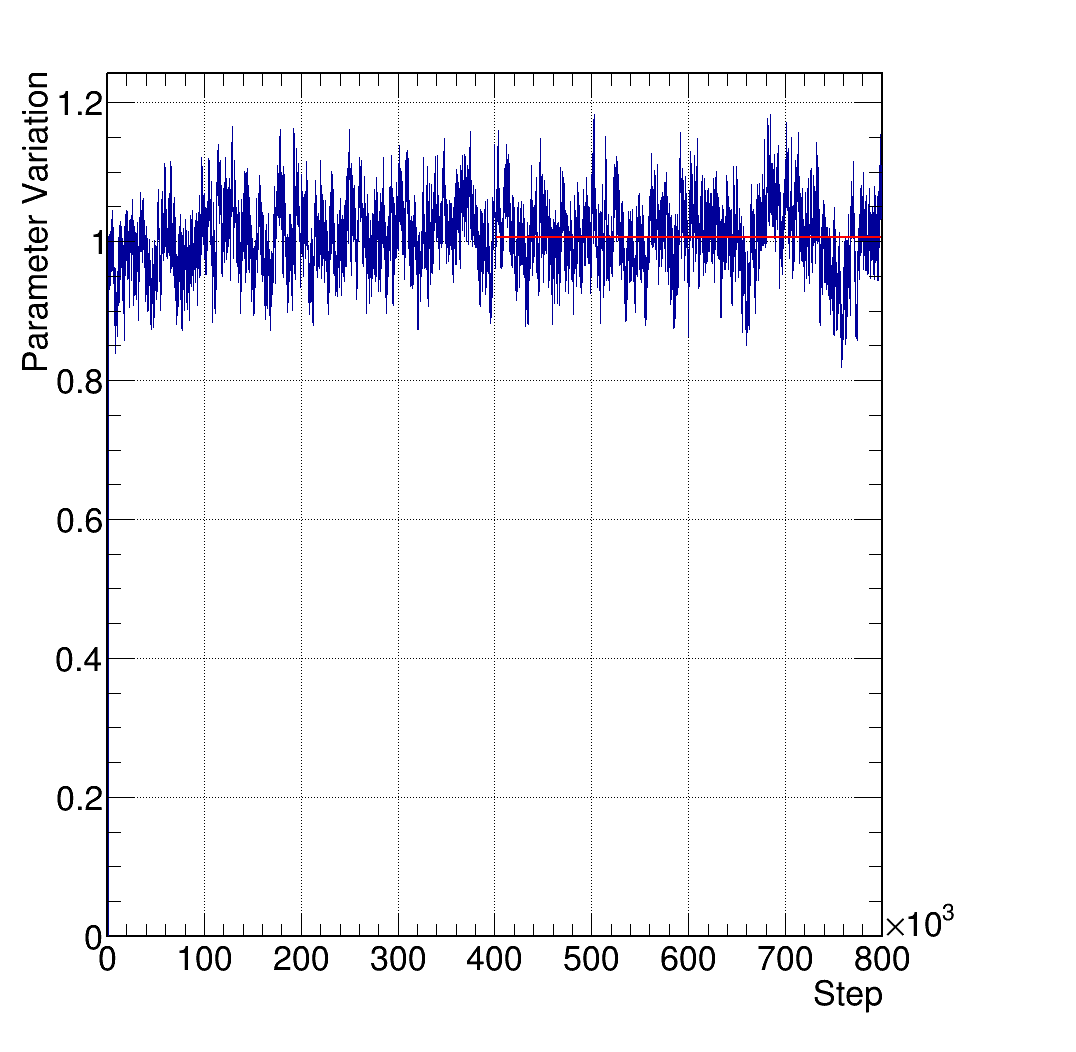
\includegraphics[width=0.73\linewidth]{figs/trace0}
  \caption{Step Size Scale: 0.03}
  \label{fig:trace0}
\end{subfigure}%
\begin{subfigure}{.5\textwidth}
  \centering
  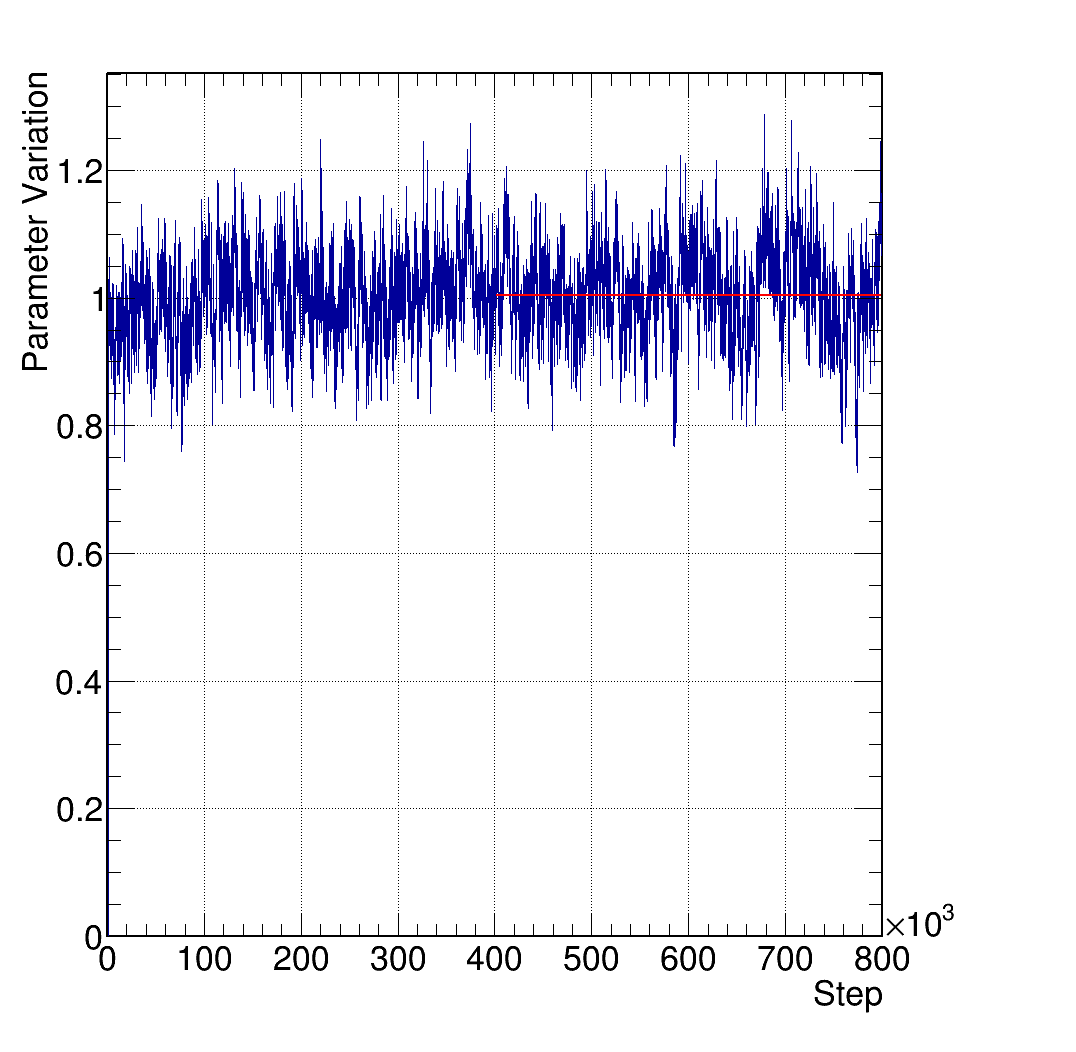
\includegraphics[width=0.73\linewidth]{figs/trace1}
  \caption{Step Size Scale: 0.04}
  \label{fig:trace1}
\end{subfigure} \\
\begin{subfigure}{.5\textwidth}
  \centering
  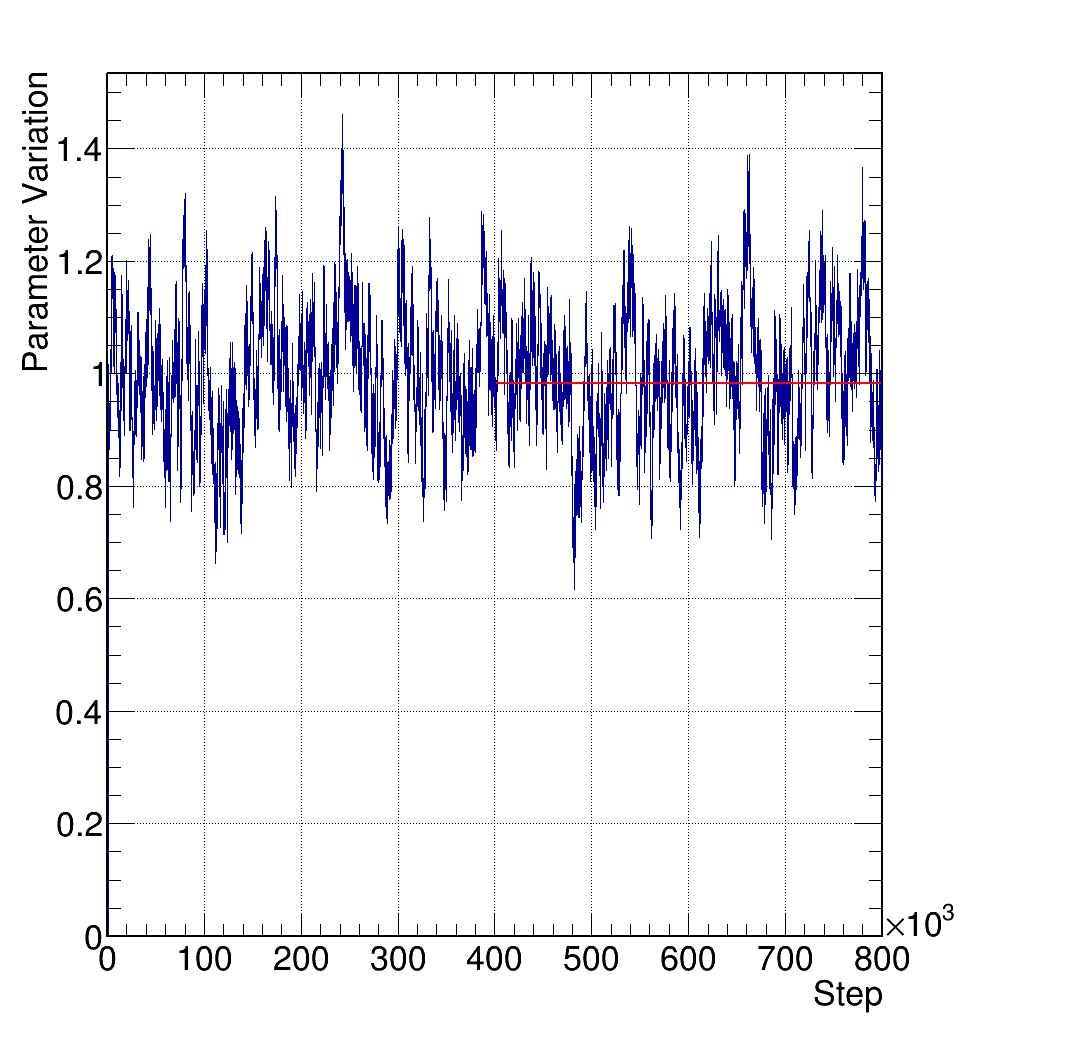
\includegraphics[width=0.73\linewidth]{figs/trace2}
  \caption{Step Size Scale: 0.075}
  \label{fig:trace2}
\end{subfigure}%
\begin{subfigure}{.5\textwidth}
  \centering
  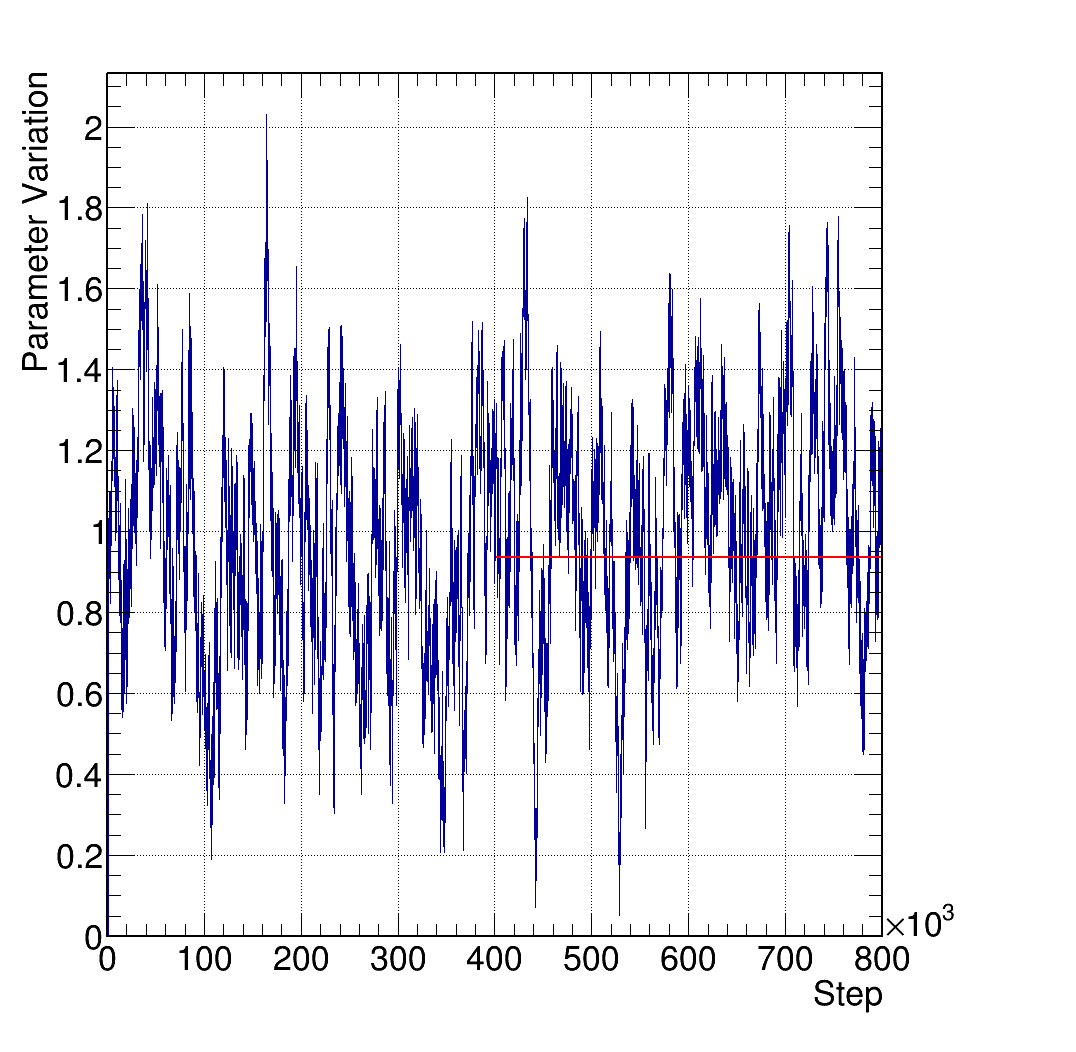
\includegraphics[width=0.73\linewidth]{figs/trace3}
  \caption{Step Size Scale: 0.10}
  \label{fig:trace3}
\end{subfigure}
\caption{The traces for a low energy flux parameter for different scalings of the step size. The red lines show the mean for the second half of the chain.}
\label{fig:traces}
\end{figure}

Finally, batched means are also used to test the chain has converged. These are the mean of a given parameter over smaller consecutive subsets of steps. Once converged, these should be fairly constant, as shown in Figure \ref{fig:batch} for a low energy flux parameter. In the second half of the chain, the batched means are within $\sim$2$\%$. If the mean was varying drastically between batches, or if there were regions of consistent bias beyond statistical fluctuation, it would suggest the stationary distribution had not been reached.

\begin{figure}[!htbp]
\centering
\includegraphics*[width=0.8\textwidth,clip]{figs/batch}
\caption{The batched means for a low energy flux at parameter. The red line shows the total mean.}\label{fig:batch}
\end{figure}

In this analysis, the general method used for step size tuning was to individually alter the width of the proposal function for each individual cross-section parameter until the autocorrelations were similar for all parameters. Then a further global scaling was applied to achieve the desired acceptance rate. Step size tuning, however, is not an exact science. When trying to reduce one parameter's autocorrelation, another parameter's could unexpectedly increase due to high dimensional correlations. One could always endeavour to further reduce autocorrelations, but once a reasonable set of tunings was found with good mixing, fairly consistent autocorrelations, and an acceptance rate close to the optimal value, no further time was spent trying to tune further.

Even with a well tuned Markov Chain, it is still desirable to run for as many steps as possible, to ensure good coverage. In this analysis, six chains of 800,000 steps were run in parallel and then merged. However, not all steps are used in the final results. As the initial values of parameters in the chain are not necessarily in a region of high posterior probability, there is a `burn-in' period before the chain reaches its stationary distribution.

The batched means and traces for individual parameters can be used to monitor the number of steps in the burn-in. Figure \ref{fig:batch} shows the means initially being lower than the final converged values, while Figure \ref{fig:burnin} shows the parameter value starting higher than it's final value, but quickly converging after 10,000 steps and then exploring the surrounding region. 

\begin{figure}[!htbp]
\centering
\includegraphics*[width=0.8\textwidth,clip]{figs/burnin}
\caption{The trace of the first 50,000 steps of high energy flux parameter, showing the initial burn-in phase before reaching the stationary distribution.}\label{fig:burnin}
\end{figure}

The trace of the systematic and sample contributions to the log-likelihood are also a good measure of when the burn-in period has finished. These are shown in Figure \ref{fig:llhs}, for six merged chains each with 600,000 steps. The negative log-likelihoods converge once the stationary distribution has been reached after $\sim$20,000 steps.

\begin{figure}
\centering
\begin{subfigure}{.5\textwidth}
  \centering
  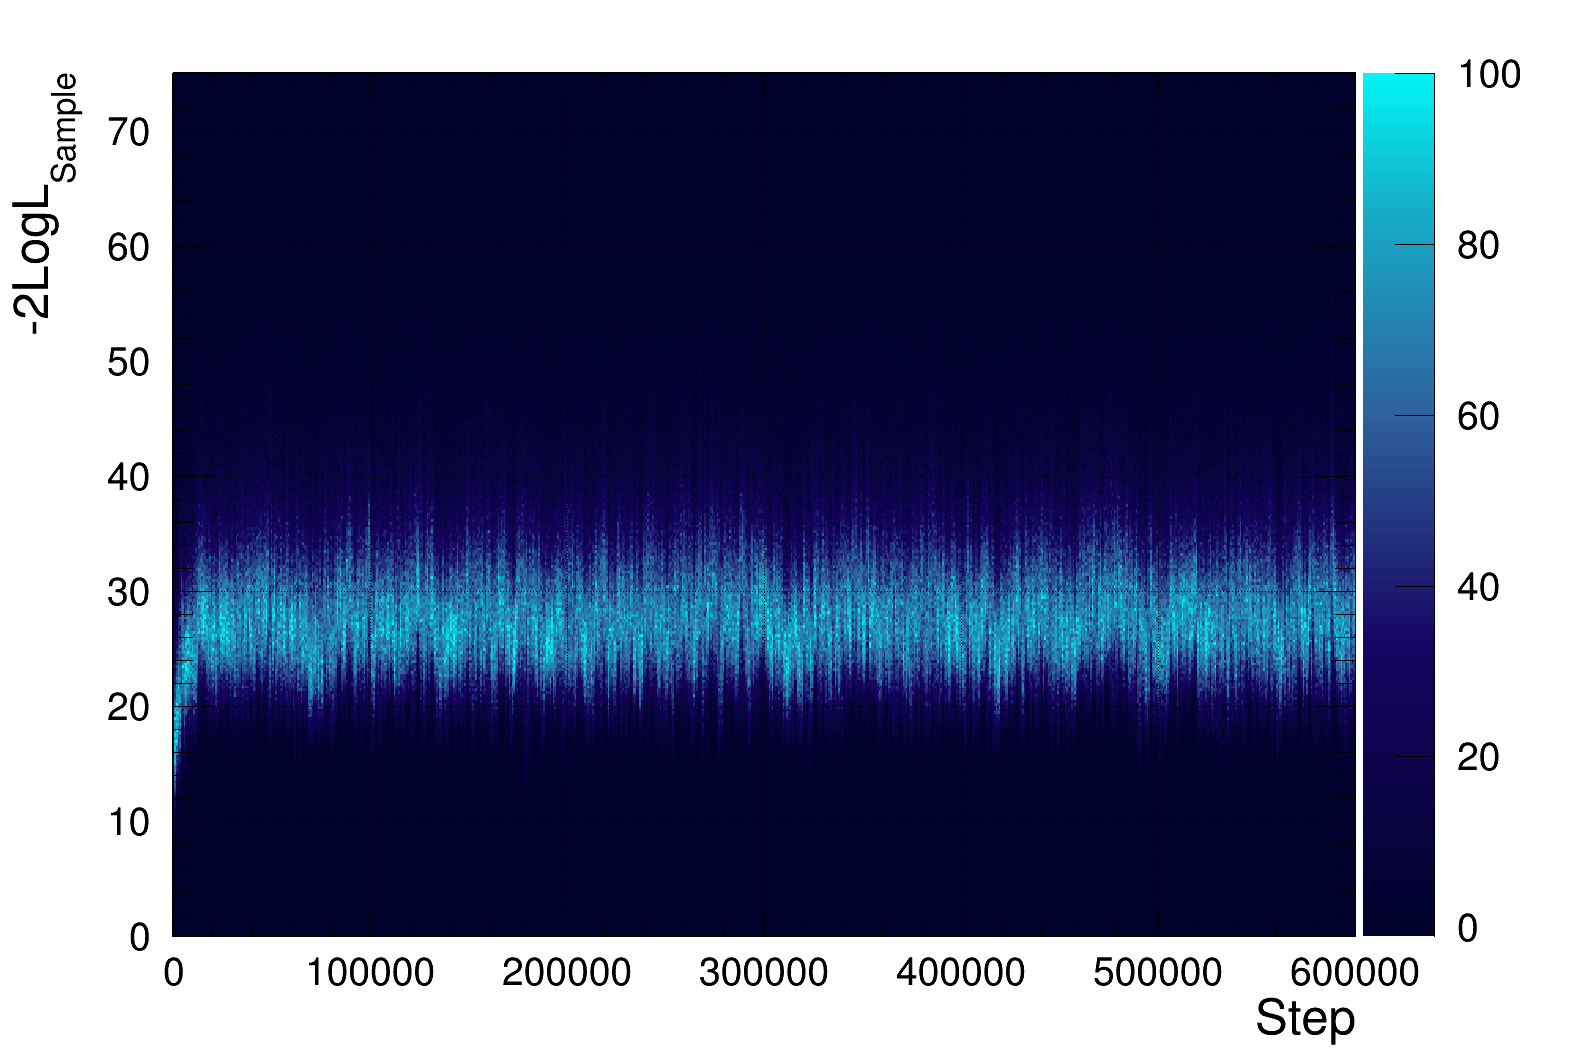
\includegraphics[width=0.85\linewidth]{figs/llh_sam}
  \caption{Sample contribution}
\end{subfigure}%
\begin{subfigure}{.5\textwidth}
  \centering
  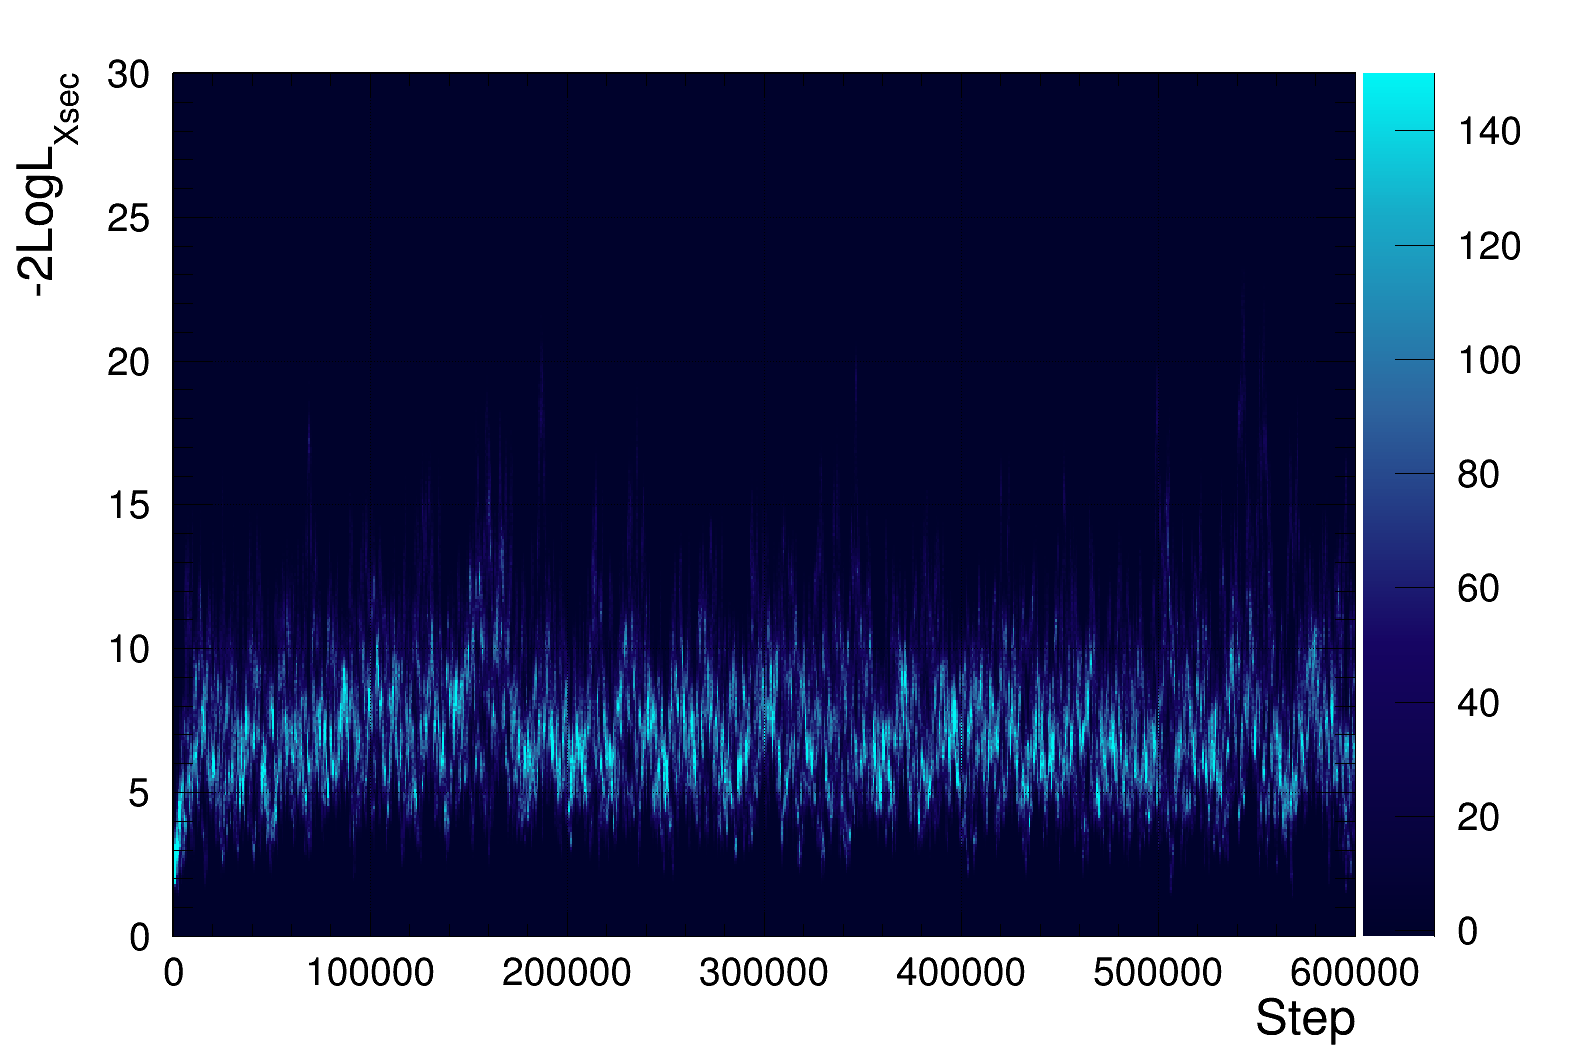
\includegraphics[width=0.85\linewidth]{figs/llh_xsec}
  \caption{Cross-section penalty contribution}
\end{subfigure} \\
\begin{subfigure}{.5\textwidth}
  \centering
  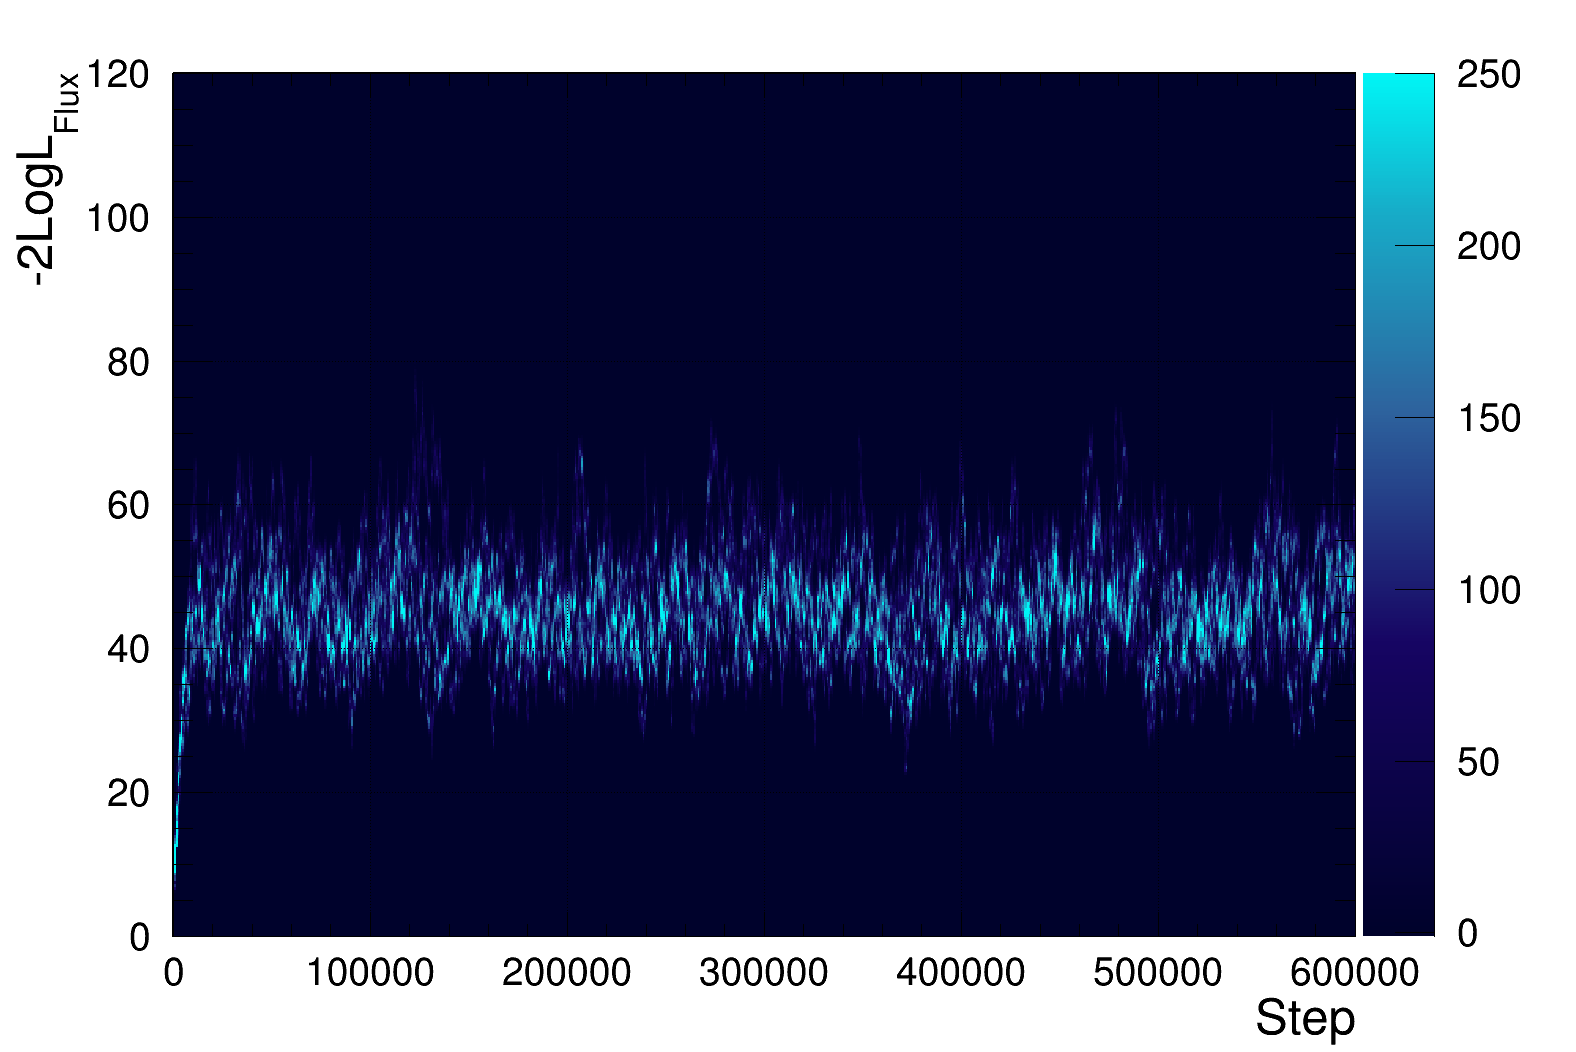
\includegraphics[width=0.85\linewidth]{figs/llh_flux}
  \caption{Flux penalty contribution}
\end{subfigure}%
\begin{subfigure}{.5\textwidth}
  \centering
  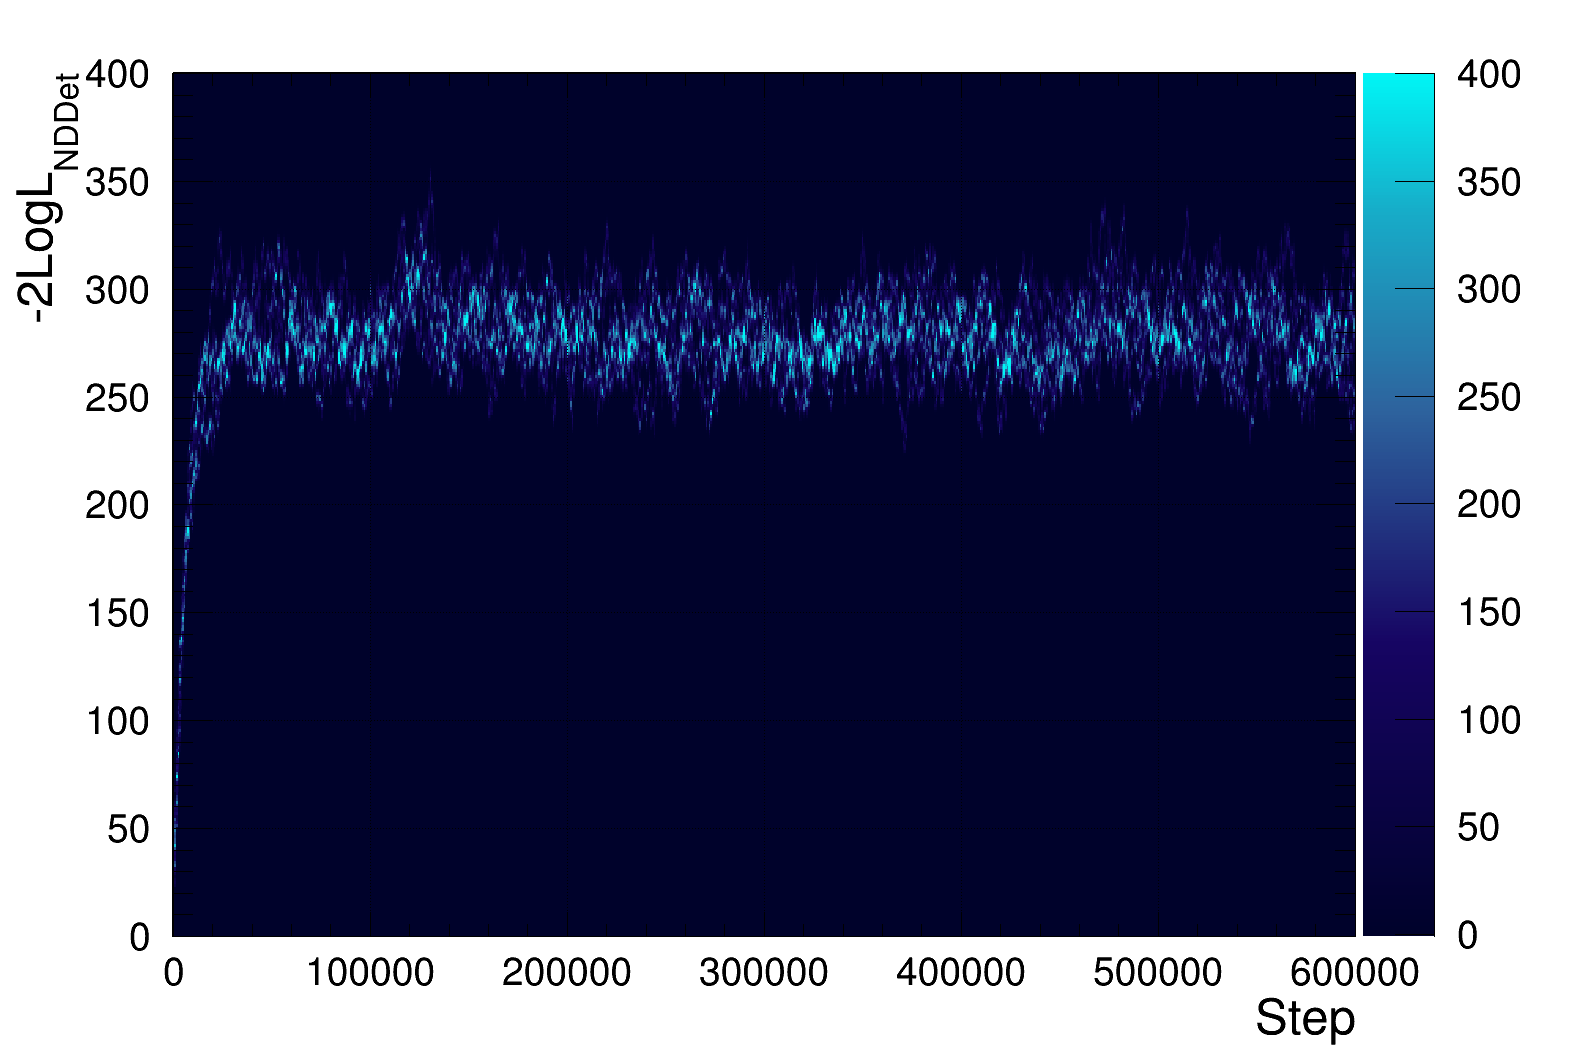
\includegraphics[width=0.85\linewidth]{figs/llh_nddet}
  \caption{Detector penalty contribution}
\end{subfigure}
\caption{Trace of the different contributions to the LLH for 6 merged chains each of 600,000 steps in total. The LLHs all converge within $\sim$20,000 steps, though 150,000 are rejected as burn-in to ensure the stationary distribution has been reached.}
\label{fig:llhs}
\end{figure}

In general, a large amount of steps from the start of the chain should be rejected, to ensure convergence has been reached for all the steps used. In this analysis, the first 1/4 of steps of all chains are conservatively cut out as burn-in.

\section{Postfit Treatment}\label{sec:postfit}

In this analysis, the full $\sim$700 dimensional posterior distribution is the final result which is propagated to the detector. However, interpreting the results for validations before joint fits is not feasible in this high a number of dimensions. Therefore information needs to be removed to be able to intuitively understand the results. 

\subsection{Parameter Value Extraction}\label{sec:extrac}

Interpreting individual parameter behaviour is achieved by marginalising over all parameters but one, one by one. This is equivalent to integrating the posterior distribution over all parameters but a single parameter of interest. For a parameter $\theta_i$ of model $\bar{\theta}$, the marginalised posterior given data, \textit{D}, is given by:

\begin{equation}
P(\theta|D) = \int P(\bar{\theta}',\theta_i|D)d\bar{\theta}',
\end{equation}

where $\bar{\theta}'$ is the parameter space over all model parameters but $\theta_i$.

Figure \ref{fig:1dposts} shows the resulting 1-dimensional projections for two individual fit parameters. This is equivalent to the parameter value at each step in the Markov Chain after burn-in. Central values and uncertainties for each parameter are extracted by three different methods. Firstly, the arithmetic mean and RMS of the histogram are calculated and used as the postfit parameter value and error. Secondly, the highest posterior density, or mode, of the histogram is taken as the central value. The number of events in each bin is summed outwards from the mode to obtain an asymmetric uncertainty. Finally, a Gaussian is fitted to the histogram and its mean and width are taken as the central value and uncertainty.

\begin{figure}
\centering
\begin{subfigure}{.5\textwidth}
  \centering
  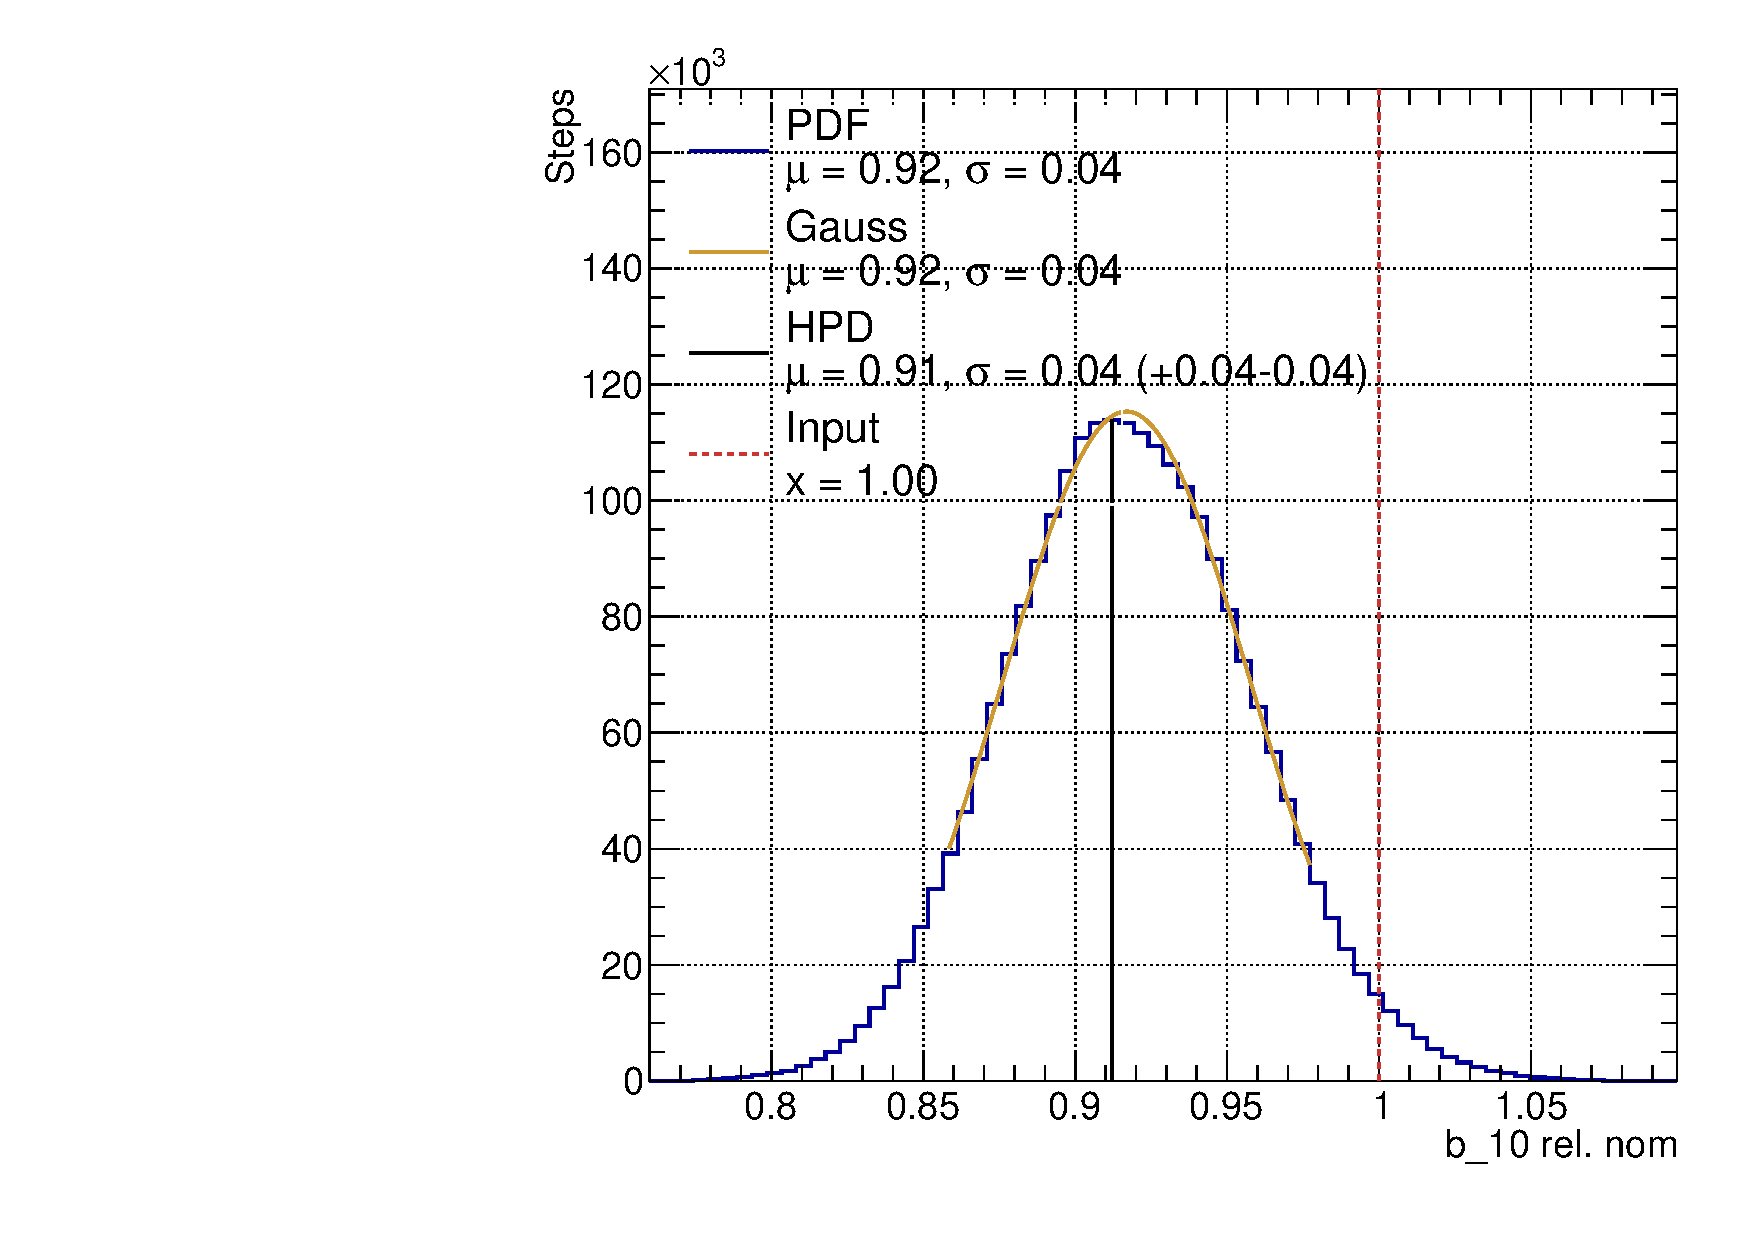
\includegraphics[width=0.95\linewidth]{figs/b_10}
  \caption{A high energy FHC near detector flux parameter.}
  \label{fig:b10}
\end{subfigure}%
\begin{subfigure}{.5\textwidth}
  \centering
  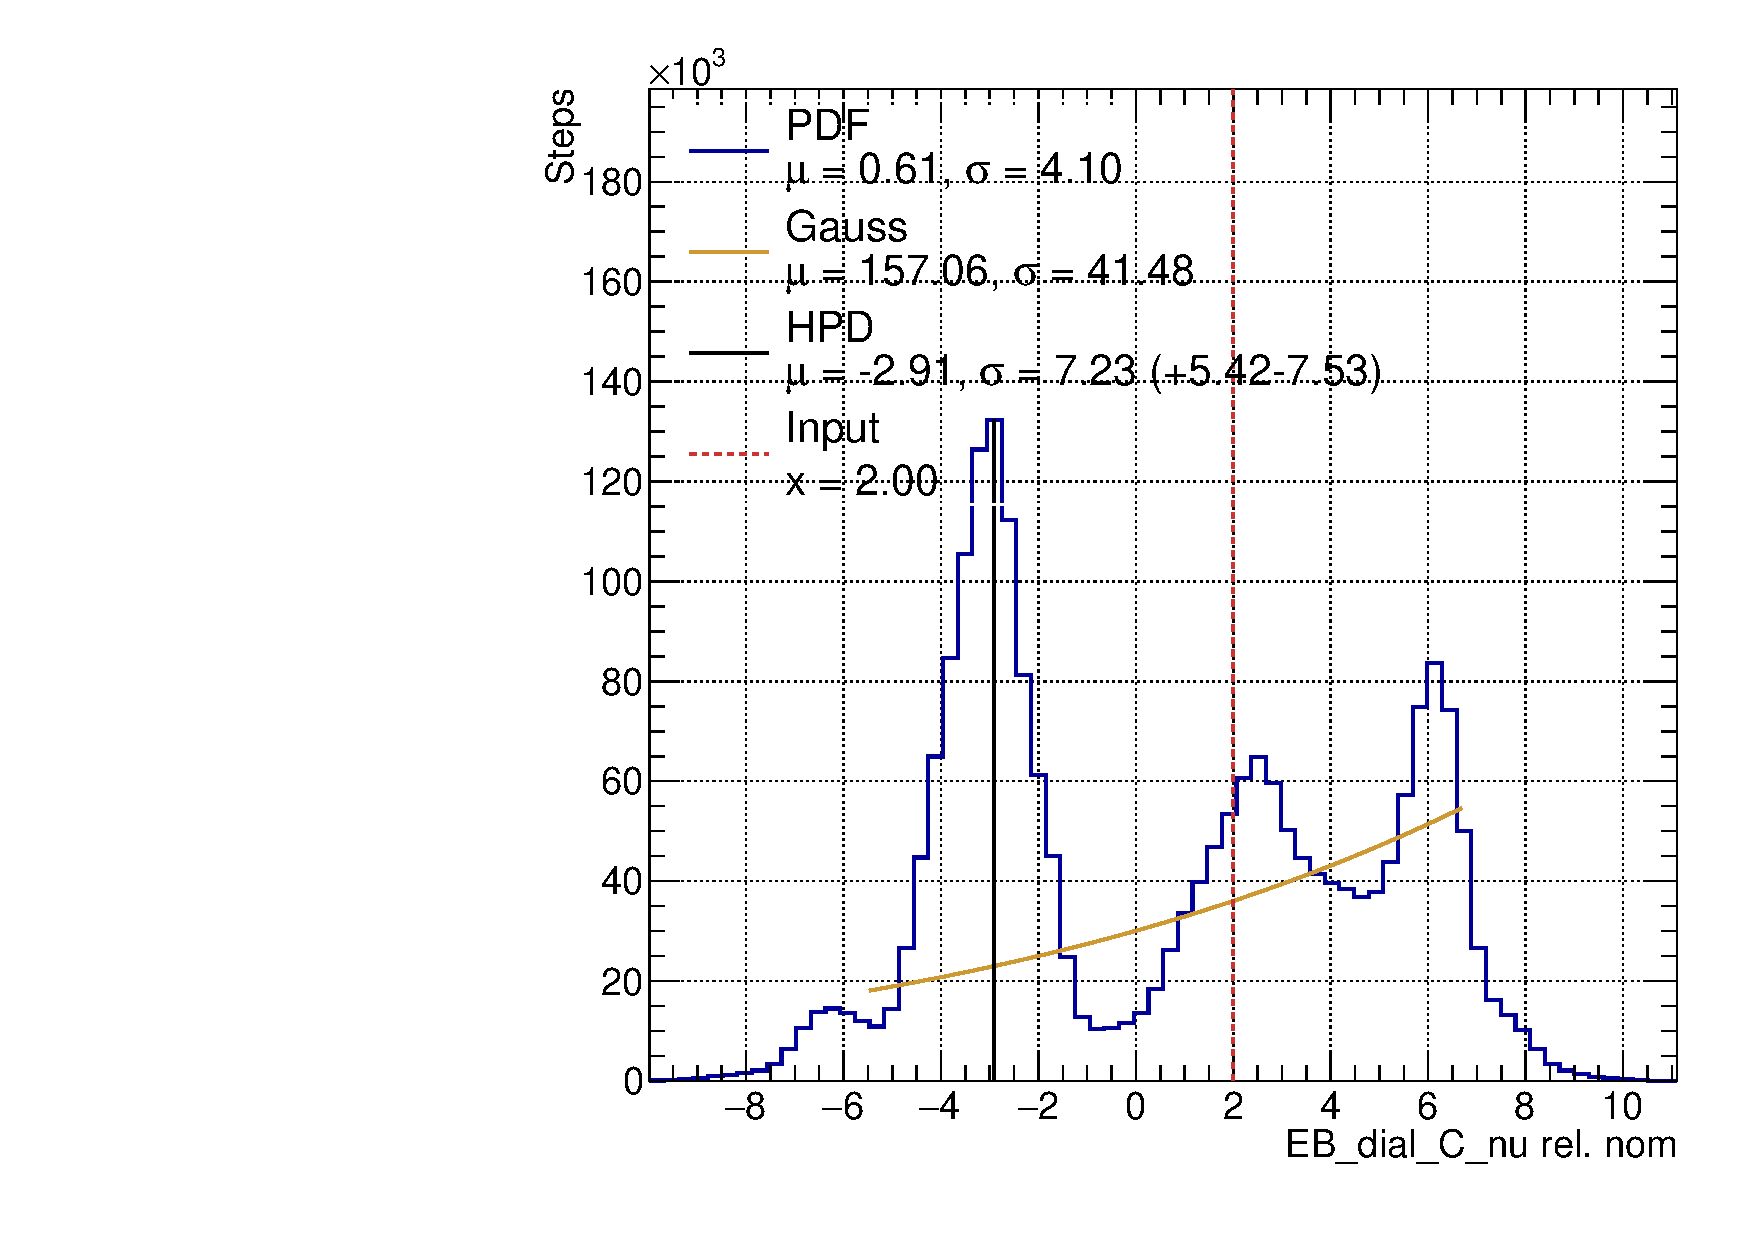
\includegraphics[width=0.95\linewidth]{figs/EB_dial_C_nuData}
  \caption{The binding energy parameter for neutrino interactions on carbon.}
  \label{fig:Eb}
\end{subfigure}
\caption{The 1-dimensional marginalised distribution for two fit parameters, showing the different methods of parameter extraction. The red lines show the prior central values, the gold lines show the fitted Gaussian distributions, and the black lines show the highest posterior density point.}
\label{fig:1dposts}
\end{figure}

For a Gaussian distribution these three methods are equivalent, as shown in Figure \ref{fig:b10}. However, non-Gaussian distributions and parameter correlations can lead to non-intuitive results when marginalised over, moving the region of high probability in the marginal posterior distribution. This is an expected, true effect, which does not indicate any bias in the fit. The three extracted values are compared to each other, with any differences highlighting non-Gaussian behaviour, as shown in Figure \ref{fig:Eb}. Non-Gaussianity is not necessarily concerning, but should be understood and considered when interpreting other parameter results. 

None of the three extraction methods are incorrect, but none of them contain the whole true result either. Only the full $\sim$700 dimensional distribution contains all the information of the final fit result. As this is what is propagated to SK, differences between the extracted 1D values is not an issue in itself. 

The postfit values are also compared to those from the other T2K near detector fitting groups for validation. As the other group finds the single set of parameter values to minimise the test statistic, some differences are expected from marginalisation over non-Gaussian and correlated distributions. However, large discrepancies could indicate differences between the implementation of the fit in the two groups.

\subsection{Postfit Covariance}\label{sec:postcov}

A similar process is used to calculate the postfit covariance between parameters. All parameters are marginalised over but two, and this is repeated until each combination of two parameters have been projected onto. Figure \ref{fig:corrs} shows this for two pairs of parameters. This is equivalent to the values of each parameter at each step of the Markov Chain post burn-in. The covariance between the two parameters of interest is calculated from the arithmetic width of the distribution. This is the only method used to extract the covariance, as no shape is assumed for the 2-dimensional posterior.

\begin{figure}
\centering
\begin{subfigure}{.5\textwidth}
  \centering
  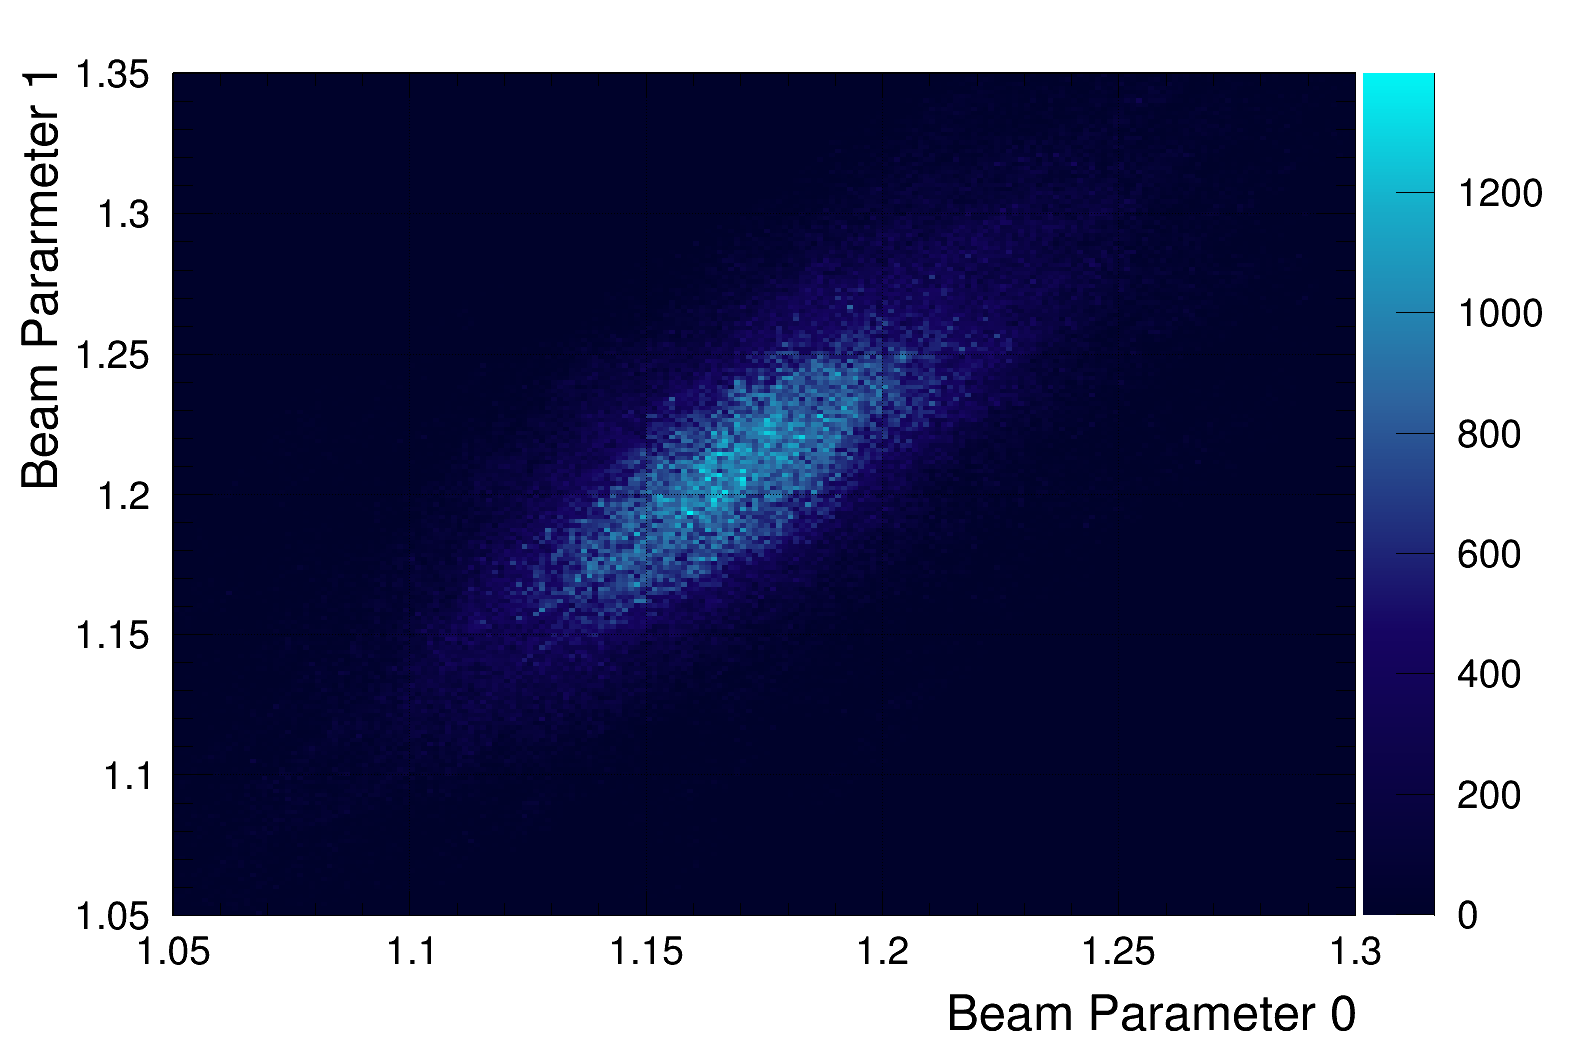
\includegraphics[width=0.95\linewidth]{figs/corr1}
  \caption{Two highly correlated beam parameters.}
  \label{fig:corr1}
\end{subfigure}%
\begin{subfigure}{.5\textwidth}
  \centering
  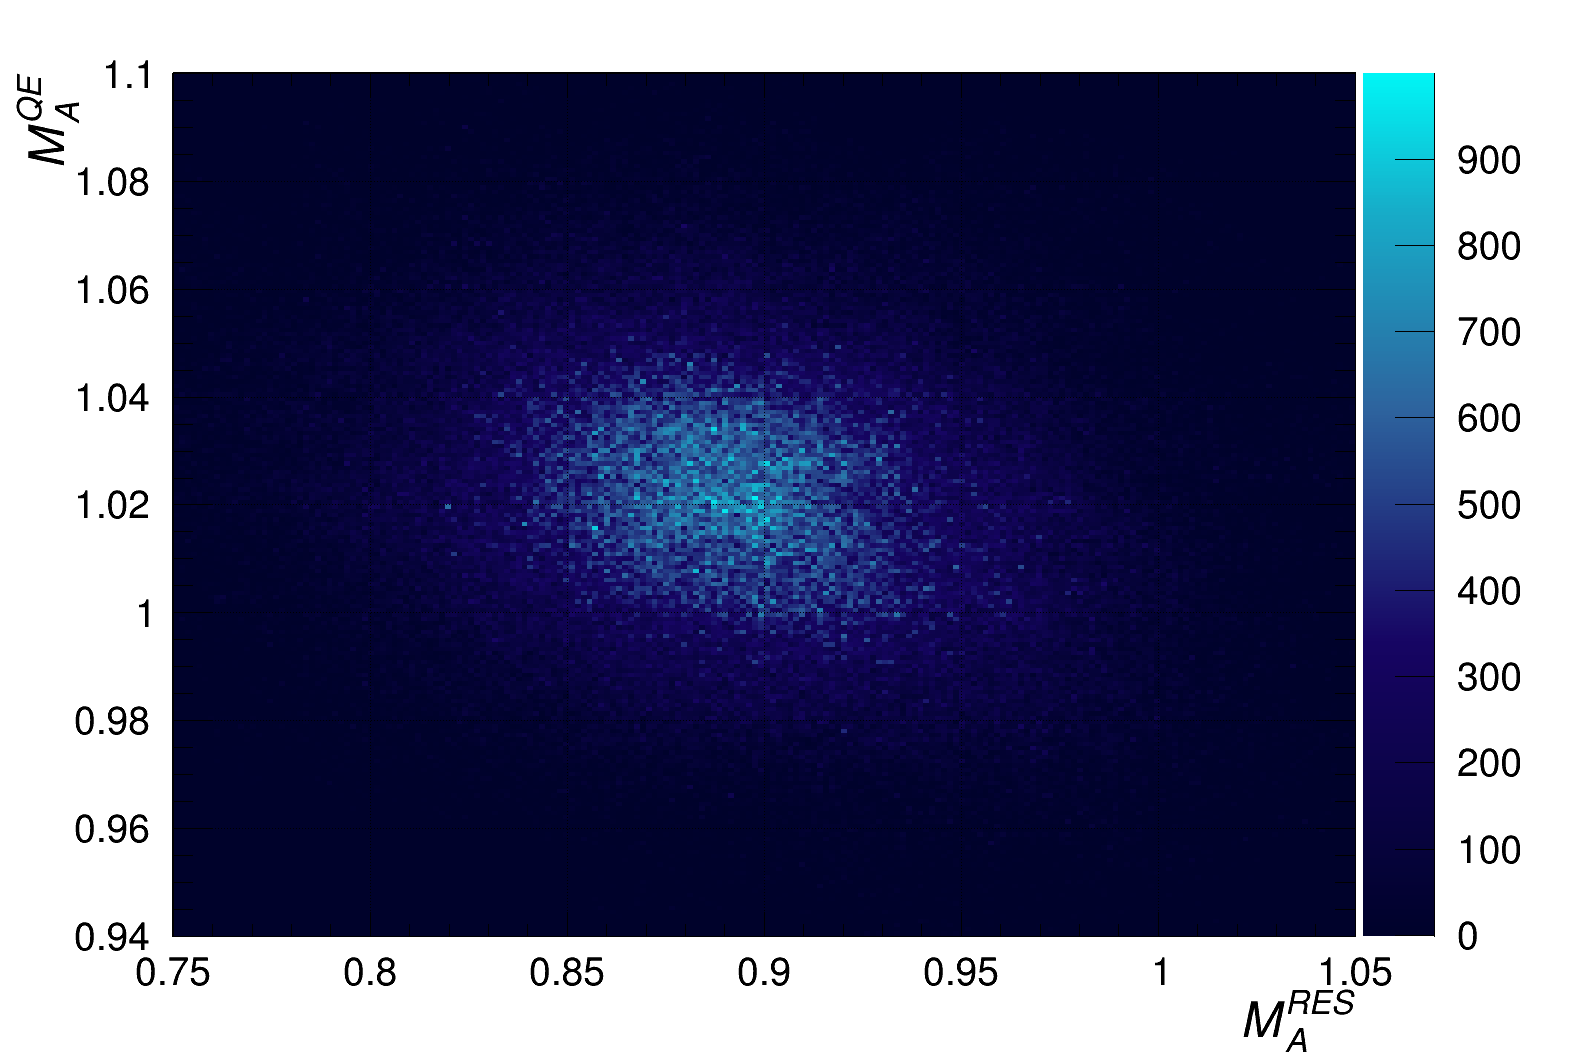
\includegraphics[width=0.95\linewidth]{figs/corr2}
  \caption{Two less correlated interaction parameters.}
  \label{fig:corr2}
\end{subfigure}
\caption{The 2-dimensional marginalised distributions for two pairs of fit parameters.}
\label{fig:corrs}
\end{figure}

Although reducing each of these 2-dimensional marginal posteriors to a single number removes information, the covariances are only used for comparisons with the other near detector fitting group and to highlight unexpected strong intra-parameter correlations. The full $\sim$700 dimensional posterior distribution is all that is propagated to the far detector analysis.

\subsection{Posterior Predictions}\label{sec:postpred}

Once the fit has finished, the results are used to produce the posterior predictive distributions with the final fitted parameters. However, as discussed in the previous sections, just marginalising over all but one parameter, one by one, removes significant information from the full posterior. Although this is useful for intuitively interpreting the fit, removing information is not necessary for producing postfit event distributions. The method used in this analysis is as follows:

\begin{itemize}
   \item Draw 2000 post burn-in steps from the Markov Chain
   \item For each draw, reweight the MC to the set of parameter values for that step. For each fit bin in each sample, this gives 2000 different number of events
   \item Fit a Gaussian to the distribution of number of events from all draws in each fit bin 
   \item For each bin in each sample, the mean and width of the fitted Gaussian become the central value and uncertainty for the posterior prediction
   \end{itemize}
   
In this way, a predictive distribution representative of the draws from the stationary distribution is produced. The comparison of this prediction to the data can be used to see if the model has enough freedom to closely reproduce the data through reweighting. Furthermore, plotting the log-likelihood (LLH) contribution from the posterior prediction to data for each bin in each sample highlights which regions are affecting the LLH calculation the most. It is desired that bins containing the most bins would be having the largest impact on the fit, and when this is not the case it should be fully understood why other regions are having unexpected significance. However, more involved methods are needed to truly test how well the model has been fit to the data.

\subsection{Goodness of Fit}\label{sec:pval}

In this analysis, the distribution of fitted model parameters to data is found. However, this only determines how best to describe the data using the implemented model. If the model does not agree well with the data misleading results can be produced. It is therefore important to be able to assess the goodness of fit for the final result.

As well as comparing the posterior predictive distributions to data, a Bayesian p-value is calculated to see how well the model fits the data. This is done in accordance with the methods outlined in \cite{Gelman_Example,Gelman_Post,Gelman_Understanding}.  The 2000 draws used to produce the posterior predictions are used:

\begin{itemize}
	\item For each fit bin in each sample, the bin contents in the posterior prediction is fluctuated by drawing a random number from a Poisson distribution with a mean equal to the original bin content
	\item Calculate the LLH between the fluctuated prediction and the prediction
   \item For each draw:
   \begin{itemize}
   \item Reweight the MC to the set of parameter values for that step
   \item Calculate the LLH between the data and the draw
   \item For each fit bin in each sample, the bin contents for the draw is fluctuated by drawing a random number from a Poisson distribution with a mean equal to the original bin content
  \item Calculate the LLH between the fluctuated draw and the draw
  \end{itemize}
\end{itemize}

The LLHs are calculated using Equation \ref{eqn:llhsample}. The Bayesian p-value is then calculated in two different ways:

\begin{equation}
p = \frac{N(-2LLH_{Data, Draw} < -2LLH_{Draw Fluc, Draw})}{N_{Total}},
\end{equation}

and

\begin{equation}
p = \frac{N(-2LLH_{Data, Draw} < -2LLH_{Pred Fluc, Pred})}{N_{Total}},
\end{equation}

where $N(-2LLH_{Data, Draw} < -2LLH_{Draw Fluc, Draw}$ is the number of draws for which the negative LLH is smaller for the data given the draw than for the fluctuation of the draw given the draw, $N(-2LLH_{Data, Draw} < -2LLH_{Pred Fluc, Pred})$ is the number of draws for which the negative LLH is smaller for the data given the draw than for the posterior prediction given the fluctuated posterior prediction, and $N_{Total}$ is the total number of draws. The first method gives a measure of how likely we would be to have observed the data we did, or something more extreme, compared to random fluctuations of the model, if the fitted model describes nature. If the selected draws are representative of the posterior distribution, the second method should produce similar p-values to the first.

The p-values can be calculated by plotting the 2-dimensional histograms of\\ $-2LLH_{Data, Draw}$ vs $-2LLH_{Draw Fluc, Draw}$ and $-2LLH_{Data, Draw}$ vs $-2LLH_{Pred Fluc, Pred}$ and calculating the proportion of steps below the line $y=x$. This is done for each sample individually, and as a total sum for all samples using the LLH contribution from every fit bin. 

Neither method of calculating the p-value is individually correct or incorrect, and neither should be interpreted as a binary measure of whether the model can or cannot describe the data. The p-values presented here should therefore not be taken as a single validation of the fit, but used along with final marginalised distribution to interpret the full results. Given that a significant amount of information has to be removed from the full $\sim$700 dimensional posterior for it to be intuitively understood, using a measure of goodness of fit alongside the marginalised distributions is useful for extracting the full picture of the fit.

Generally a higher p-value is desirable and indicates a better fit to data, but there is no single threshold for which a higher p-value can be determined acceptable for all analyses. There are also deficiencies in this method of calculating the p-value which should be considered when evaluating the goodness of fit. The detector systematics are not varied individually, but instead grouped together and parametrised by their joint effect on event rates in merged fit bins, as described in Section \ref{sec:det}. As these underlying systematics are non-Gaussian, throwing using these merged bins does not necessarily describe the true distribution of these systematics. This could cause the p-value to be lower than would otherwise be measured.

Furthermore, this Bayesian p-value is not the same as a 'traditional' p-value. Here, the p-value answers a very specific question: if the experiment was ran again, how likely is it that data consistent with the post-fit model would be observed? This is, by construction, a stringent test. As SK has much lower statistics than ND280, if this p-value is low it does not necessarily mean that the extrapolation of the near detector result to the far detector is invalid, but the individual p-values for each sample can highlight regions of phase space for which the postfit model is less compatible with the data.

The other near detector fitting group at T2K also produce a p-value, using the method described in \cite{tn324}. This is a strictly frequentist construction, calculated using throws of the systematics from their priors, giving an indication of how well the prior model can fit the data. As well as this, this p-value uses throws of the underlying detector systematics, rather than the effective bin-by-bin normalisations, giving more accurate variations. The frequentist p-value answers a different question to the Bayesian version: using information on the systematics before the fit is run, how likely is the observed data? The two p-values are therefore not expected to give the same results. For this analysis, the frequentist p-value is used to determine if an acceptable goodness of fit has been achieved, as it uses the correct detector systematics implementation, while the Bayesian p-value is used to inspect the fit result in more detail and determine for which samples and regions of phase space the fit performs well for.

\section{Summary}

This chapter has presented an overview of the statistical methods used in this analysis. Bayesian statistics are invoked, combining prior information with the likelihood of a sample, to find the set of parameter values which best describe the data.

Markov Chain Monte Carlo is used to fit the systematic uncertainties to data. The Metropolis-Hastings algorithm is used to produce a Markov Chain with a density of points proportional to the posterior probability distribution.

Extensive diagnostics are performed on the Markov Chain to ensure the stationary distribution has been reached. These include step-size tuning and inspecting the autocorrelations, batched means, parameter traces, and burn-in.

Postfit parameter values and uncertainties are extracted from the Markov Chain by three different methods. The first step is to marginalise over all but one parameter, one by one. The arithmetic mean, mode, and mean of a fitted Gaussian to the resulting 1D distribution can then all be used as the parameter's postfit result. The methods can produce different results if the distribution is non-Gaussian, but as the full $\sim700$ dimensional distribution is propagated to the far-detector, this is not problematic. The extracted single parameter values are only used for validating the fit and comparing to the other near detector fitting group. Postfit correlation matrices are also produced by marginalising over all but two parameters, for each combination of a pair of parameters.

Posterior predictions are produced by drawing 2000 steps from the Markov Chain and fitting Gaussians to the number of events in each bin, showing the $p-$cos$\theta$ distributions the postfit model produces.

Finally, the goodness of fit is calculated in two separate ways from random draws of the Markov Chain. These are not equivalent to a traditional frequentist $p$-value, and should not be interpreted as a single binary measure of whether the model can or cannot describe the data. Rather, they are used to determine for which regions of phase space the fit performs well.

\newpage